% Created by tikzDevice version 0.9 on 2016-01-08 19:27:12
% !TEX encoding = UTF-8 Unicode
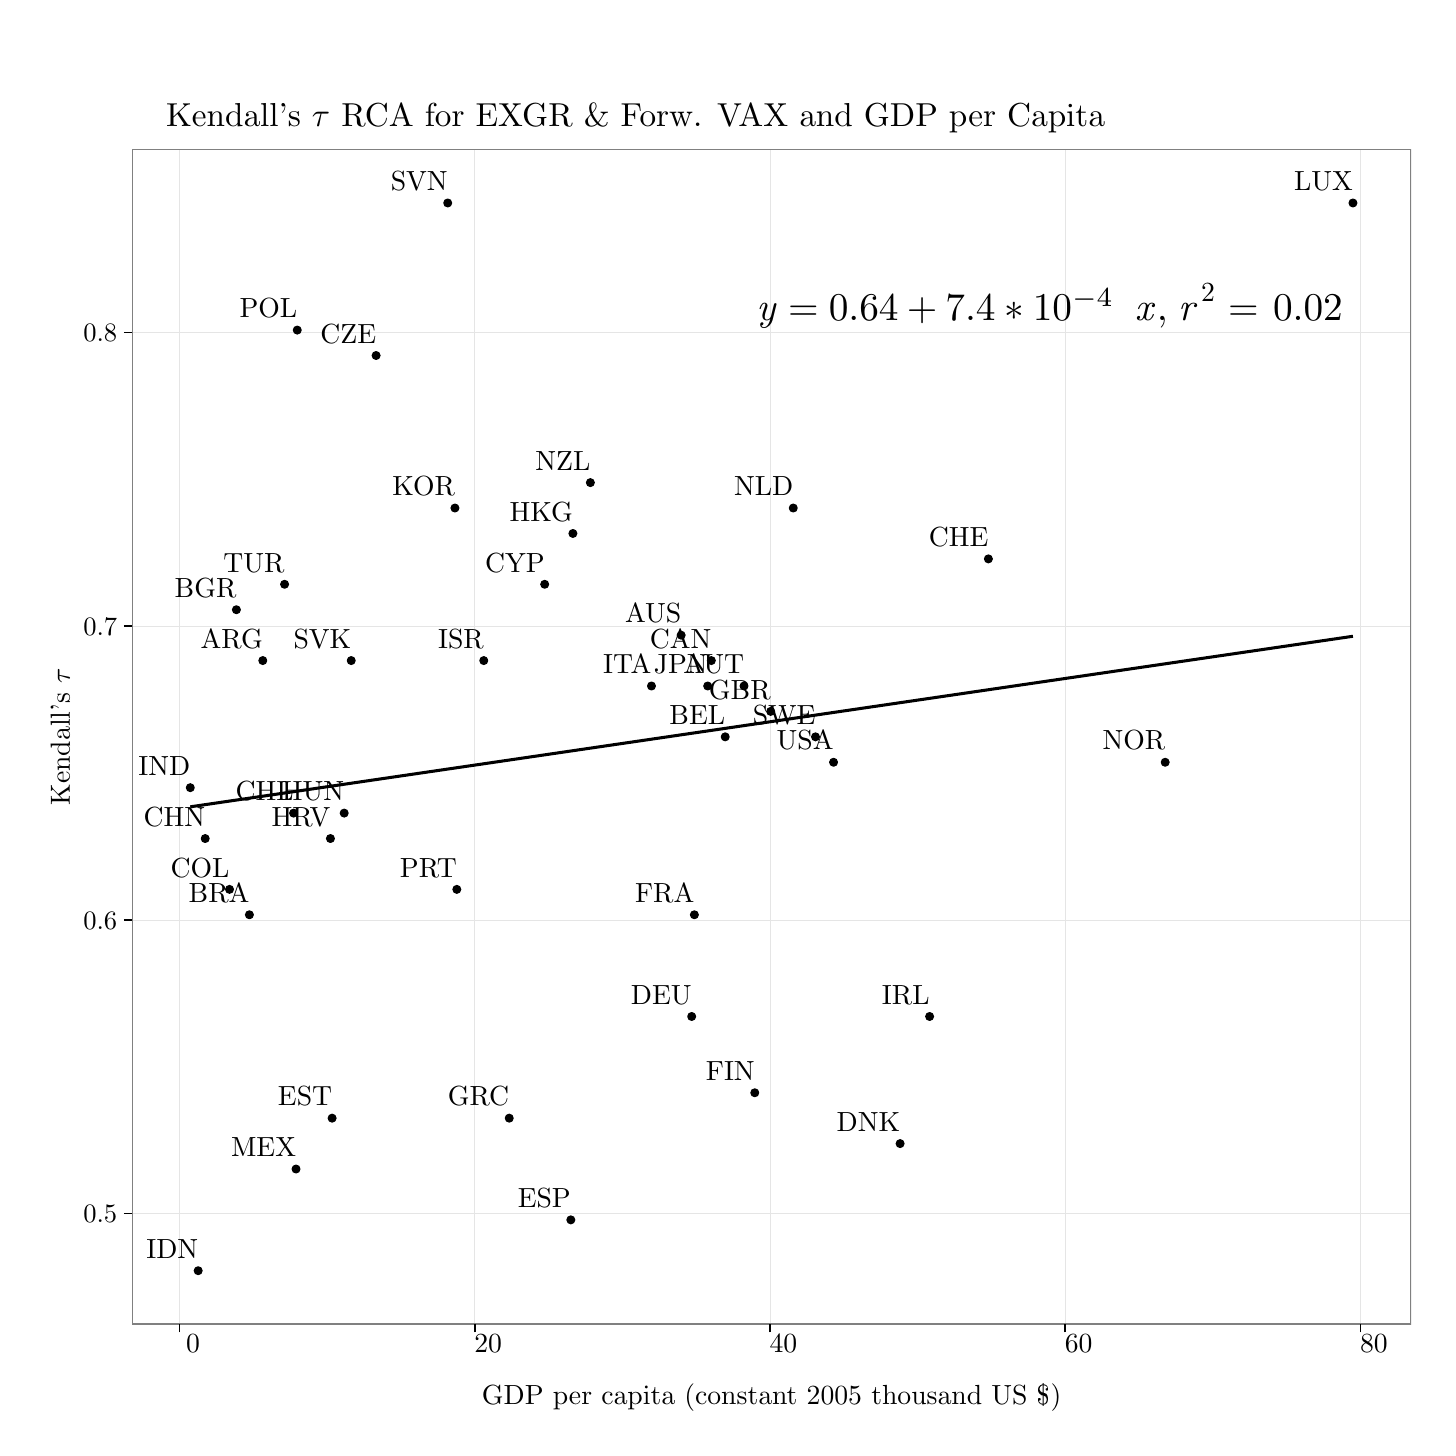
\begin{tikzpicture}[x=1pt,y=1pt]
\definecolor{fillColor}{RGB}{255,255,255}
\path[use as bounding box,fill=fillColor,fill opacity=0.00] (0,0) rectangle (505.89,505.89);
\begin{scope}
\path[clip] (  0.00,  0.00) rectangle (505.89,505.89);
\definecolor{drawColor}{RGB}{255,255,255}
\definecolor{fillColor}{RGB}{255,255,255}

\path[draw=drawColor,line width= 0.6pt,line join=round,line cap=round,fill=fillColor] (  0.00, -0.00) rectangle (505.89,505.89);
\end{scope}
\begin{scope}
\path[clip] ( 37.75, 37.43) rectangle (499.89,461.83);
\definecolor{fillColor}{RGB}{255,255,255}

\path[fill=fillColor] ( 37.75, 37.43) rectangle (499.89,461.83);
\definecolor{drawColor}{gray}{0.90}

\path[draw=drawColor,line width= 0.2pt,line join=round] ( 37.75, 77.39) --
	(499.89, 77.39);

\path[draw=drawColor,line width= 0.2pt,line join=round] ( 37.75,183.49) --
	(499.89,183.49);

\path[draw=drawColor,line width= 0.2pt,line join=round] ( 37.75,289.59) --
	(499.89,289.59);

\path[draw=drawColor,line width= 0.2pt,line join=round] ( 37.75,395.69) --
	(499.89,395.69);

\path[draw=drawColor,line width= 0.2pt,line join=round] ( 54.87, 37.43) --
	( 54.87,461.83);

\path[draw=drawColor,line width= 0.2pt,line join=round] (161.55, 37.43) --
	(161.55,461.83);

\path[draw=drawColor,line width= 0.2pt,line join=round] (268.23, 37.43) --
	(268.23,461.83);

\path[draw=drawColor,line width= 0.2pt,line join=round] (374.90, 37.43) --
	(374.90,461.83);

\path[draw=drawColor,line width= 0.2pt,line join=round] (481.58, 37.43) --
	(481.58,461.83);
\definecolor{drawColor}{RGB}{0,0,0}
\definecolor{fillColor}{RGB}{0,0,0}

\path[draw=drawColor,line width= 0.4pt,line join=round,line cap=round,fill=fillColor] ( 84.96,277.19) circle( 1.42);

\path[draw=drawColor,line width= 0.4pt,line join=round,line cap=round,fill=fillColor] (236.13,286.37) circle (  1.42);

\path[draw=drawColor,line width= 0.4pt,line join=round,line cap=round,fill=fillColor] (258.85,268.00) circle (  1.42);

\path[draw=drawColor,line width= 0.4pt,line join=round,line cap=round,fill=fillColor] (252.05,249.63) circle (  1.42);

\path[draw=drawColor,line width= 0.4pt,line join=round,line cap=round,fill=fillColor] ( 75.42,295.56) circle (  1.42);

\path[draw=drawColor,line width= 0.4pt,line join=round,line cap=round,fill=fillColor] ( 80.12,185.33) circle (  1.42);

\path[draw=drawColor,line width= 0.4pt,line join=round,line cap=round,fill=fillColor] (247.04,277.19) circle (  1.42);

\path[draw=drawColor,line width= 0.4pt,line join=round,line cap=round,fill=fillColor] (347.15,313.93) circle (  1.42);

\path[draw=drawColor,line width= 0.4pt,line join=round,line cap=round,fill=fillColor] ( 96.09,222.07) circle (  1.42);

\path[draw=drawColor,line width= 0.4pt,line join=round,line cap=round,fill=fillColor] ( 64.15,212.88) circle (  1.42);

\path[draw=drawColor,line width= 0.4pt,line join=round,line cap=round,fill=fillColor] ( 72.93,194.51) circle (  1.42);

\path[draw=drawColor,line width= 0.4pt,line join=round,line cap=round,fill=fillColor] (186.82,304.75) circle (  1.42);

\path[draw=drawColor,line width= 0.4pt,line join=round,line cap=round,fill=fillColor] (125.90,387.42) circle (  1.42);

\path[draw=drawColor,line width= 0.4pt,line join=round,line cap=round,fill=fillColor] (239.94,148.58) circle (  1.42);

\path[draw=drawColor,line width= 0.4pt,line join=round,line cap=round,fill=fillColor] (315.25,102.65) circle (  1.42);

\path[draw=drawColor,line width= 0.4pt,line join=round,line cap=round,fill=fillColor] (196.27, 75.09) circle (  1.42);

\path[draw=drawColor,line width= 0.4pt,line join=round,line cap=round,fill=fillColor] (110.01,111.84) circle (  1.42);

\path[draw=drawColor,line width= 0.4pt,line join=round,line cap=round,fill=fillColor] (262.73,121.02) circle (  1.42);

\path[draw=drawColor,line width= 0.4pt,line join=round,line cap=round,fill=fillColor] (240.91,185.33) circle (  1.42);

\path[draw=drawColor,line width= 0.4pt,line join=round,line cap=round,fill=fillColor] (268.48,258.82) circle (  1.42);

\path[draw=drawColor,line width= 0.4pt,line join=round,line cap=round,fill=fillColor] (174.01,111.84) circle (  1.42);

\path[draw=drawColor,line width= 0.4pt,line join=round,line cap=round,fill=fillColor] (197.02,323.12) circle (  1.42);

\path[draw=drawColor,line width= 0.4pt,line join=round,line cap=round,fill=fillColor] (109.40,212.88) circle (  1.42);

\path[draw=drawColor,line width= 0.4pt,line join=round,line cap=round,fill=fillColor] (114.37,222.07) circle (  1.42);

\path[draw=drawColor,line width= 0.4pt,line join=round,line cap=round,fill=fillColor] ( 61.61, 56.72) circle (  1.42);

\path[draw=drawColor,line width= 0.4pt,line join=round,line cap=round,fill=fillColor] ( 58.76,231.26) circle (  1.42);

\path[draw=drawColor,line width= 0.4pt,line join=round,line cap=round,fill=fillColor] (325.91,148.58) circle (  1.42);

\path[draw=drawColor,line width= 0.4pt,line join=round,line cap=round,fill=fillColor] (164.81,277.19) circle (  1.42);

\path[draw=drawColor,line width= 0.4pt,line join=round,line cap=round,fill=fillColor] (225.41,268.00) circle (  1.42);

\path[draw=drawColor,line width= 0.4pt,line join=round,line cap=round,fill=fillColor] (245.72,268.00) circle (  1.42);

\path[draw=drawColor,line width= 0.4pt,line join=round,line cap=round,fill=fillColor] (154.39,332.31) circle (  1.42);

\path[draw=drawColor,line width= 0.4pt,line join=round,line cap=round,fill=fillColor] (478.88,442.54) circle (  1.42);

\path[draw=drawColor,line width= 0.4pt,line join=round,line cap=round,fill=fillColor] ( 96.97, 93.46) circle (  1.42);

\path[draw=drawColor,line width= 0.4pt,line join=round,line cap=round,fill=fillColor] (276.64,332.31) circle (  1.42);

\path[draw=drawColor,line width= 0.4pt,line join=round,line cap=round,fill=fillColor] (411.04,240.44) circle (  1.42);

\path[draw=drawColor,line width= 0.4pt,line join=round,line cap=round,fill=fillColor] (203.33,341.49) circle (  1.42);

\path[draw=drawColor,line width= 0.4pt,line join=round,line cap=round,fill=fillColor] ( 97.41,396.61) circle (  1.42);

\path[draw=drawColor,line width= 0.4pt,line join=round,line cap=round,fill=fillColor] (155.07,194.51) circle (  1.42);

\path[draw=drawColor,line width= 0.4pt,line join=round,line cap=round,fill=fillColor] (116.91,277.19) circle (  1.42);

\path[draw=drawColor,line width= 0.4pt,line join=round,line cap=round,fill=fillColor] (151.78,442.54) circle (  1.42);

\path[draw=drawColor,line width= 0.4pt,line join=round,line cap=round,fill=fillColor] (284.68,249.63) circle (  1.42);

\path[draw=drawColor,line width= 0.4pt,line join=round,line cap=round,fill=fillColor] ( 92.83,304.75) circle (  1.42);

\path[draw=drawColor,line width= 0.4pt,line join=round,line cap=round,fill=fillColor] (291.20,240.44) circle (  1.42);

\node[text=drawColor,anchor=base east,inner sep=0pt, outer sep=0pt, scale=  1] at ( 84.96,281.63) {ARG};

\node[text=drawColor,anchor=base east,inner sep=0pt, outer sep=0pt, scale=  1] at (236.13,290.82) {AUS};

\node[text=drawColor,anchor=base east,inner sep=0pt, outer sep=0pt, scale=  1] at (258.85,272.44) {AUT};

\node[text=drawColor,anchor=base east,inner sep=0pt, outer sep=0pt, scale=  1] at (252.05,254.07) {BEL};

\node[text=drawColor,anchor=base east,inner sep=0pt, outer sep=0pt, scale=  1] at ( 75.42,300.00) {BGR};

\node[text=drawColor,anchor=base east,inner sep=0pt, outer sep=0pt, scale=  1] at ( 80.12,189.77) {BRA};

\node[text=drawColor,anchor=base east,inner sep=0pt, outer sep=0pt, scale=  1] at (247.04,281.63) {CAN};

\node[text=drawColor,anchor=base east,inner sep=0pt, outer sep=0pt, scale=  1] at (347.15,318.38) {CHE};

\node[text=drawColor,anchor=base east,inner sep=0pt, outer sep=0pt, scale=  1] at ( 96.09,226.51) {CHL};

\node[text=drawColor,anchor=base east,inner sep=0pt, outer sep=0pt, scale=  1] at ( 64.15,217.33) {CHN};

\node[text=drawColor,anchor=base east,inner sep=0pt, outer sep=0pt, scale=  1] at ( 72.93,198.95) {COL};

\node[text=drawColor,anchor=base east,inner sep=0pt, outer sep=0pt, scale=  1] at (186.82,309.19) {CYP};

\node[text=drawColor,anchor=base east,inner sep=0pt, outer sep=0pt, scale=  1] at (125.90,391.87) {CZE};

\node[text=drawColor,anchor=base east,inner sep=0pt, outer sep=0pt, scale=  1] at (239.94,153.02) {DEU};

\node[text=drawColor,anchor=base east,inner sep=0pt, outer sep=0pt, scale=  1] at (315.25,107.09) {DNK};

\node[text=drawColor,anchor=base east,inner sep=0pt, outer sep=0pt, scale=  1] at (196.27, 79.53) {ESP};

\node[text=drawColor,anchor=base east,inner sep=0pt, outer sep=0pt, scale=  1] at (110.01,116.28) {EST};

\node[text=drawColor,anchor=base east,inner sep=0pt, outer sep=0pt, scale=  1] at (262.73,125.46) {FIN};

\node[text=drawColor,anchor=base east,inner sep=0pt, outer sep=0pt, scale=  1] at (240.91,189.77) {FRA};

\node[text=drawColor,anchor=base east,inner sep=0pt, outer sep=0pt, scale=  1] at (268.48,263.26) {GBR};

\node[text=drawColor,anchor=base east,inner sep=0pt, outer sep=0pt, scale=  1] at (174.01,116.28) {GRC};

\node[text=drawColor,anchor=base east,inner sep=0pt, outer sep=0pt, scale=  1] at (197.02,327.56) {HKG};

\node[text=drawColor,anchor=base east,inner sep=0pt, outer sep=0pt, scale=  1] at (109.40,217.33) {HRV};

\node[text=drawColor,anchor=base east,inner sep=0pt, outer sep=0pt, scale=  1] at (114.37,226.51) {HUN};

\node[text=drawColor,anchor=base east,inner sep=0pt, outer sep=0pt, scale=  1] at ( 61.61, 61.16) {IDN};

\node[text=drawColor,anchor=base east,inner sep=0pt, outer sep=0pt, scale=  1] at ( 58.76,235.70) {IND};

\node[text=drawColor,anchor=base east,inner sep=0pt, outer sep=0pt, scale=  1] at (325.91,153.02) {IRL};

\node[text=drawColor,anchor=base east,inner sep=0pt, outer sep=0pt, scale=  1] at (164.81,281.63) {ISR};

\node[text=drawColor,anchor=base east,inner sep=0pt, outer sep=0pt, scale=  1] at (225.41,272.44) {ITA};

\node[text=drawColor,anchor=base east,inner sep=0pt, outer sep=0pt, scale=  1] at (245.72,272.44) {JPN};

\node[text=drawColor,anchor=base east,inner sep=0pt, outer sep=0pt, scale=  1] at (154.39,336.75) {KOR};

\node[text=drawColor,anchor=base east,inner sep=0pt, outer sep=0pt, scale=  1] at (478.88,446.98) {LUX};

\node[text=drawColor,anchor=base east,inner sep=0pt, outer sep=0pt, scale=  1] at ( 96.97, 97.91) {MEX};

\node[text=drawColor,anchor=base east,inner sep=0pt, outer sep=0pt, scale=  1] at (276.64,336.75) {NLD};

\node[text=drawColor,anchor=base east,inner sep=0pt, outer sep=0pt, scale=  1] at (411.04,244.89) {NOR};

\node[text=drawColor,anchor=base east,inner sep=0pt, outer sep=0pt, scale=  1] at (203.33,345.93) {NZL};

\node[text=drawColor,anchor=base east,inner sep=0pt, outer sep=0pt, scale=  1] at ( 97.41,401.05) {POL};

\node[text=drawColor,anchor=base east,inner sep=0pt, outer sep=0pt, scale=  1] at (155.07,198.95) {PRT};

\node[text=drawColor,anchor=base east,inner sep=0pt, outer sep=0pt, scale=  1] at (116.91,281.63) {SVK};

\node[text=drawColor,anchor=base east,inner sep=0pt, outer sep=0pt, scale=  1] at (151.78,446.98) {SVN};

\node[text=drawColor,anchor=base east,inner sep=0pt, outer sep=0pt, scale=  1] at (284.68,254.07) {SWE};

\node[text=drawColor,anchor=base east,inner sep=0pt, outer sep=0pt, scale=  1] at ( 92.83,309.19) {TUR};

\node[text=drawColor,anchor=base east,inner sep=0pt, outer sep=0pt, scale=  1] at (291.20,244.89) {USA};

\path[draw=drawColor,line width= 1.1pt,line join=round] ( 58.76,224.34) --
	( 64.08,225.12) --
	( 69.39,225.90) --
	( 74.71,226.68) --
	( 80.03,227.46) --
	( 85.35,228.24) --
	( 90.67,229.02) --
	( 95.98,229.80) --
	(101.30,230.58) --
	(106.62,231.36) --
	(111.94,232.14) --
	(117.26,232.92) --
	(122.57,233.70) --
	(127.89,234.48) --
	(133.21,235.26) --
	(138.53,236.04) --
	(143.85,236.82) --
	(149.16,237.60) --
	(154.48,238.38) --
	(159.80,239.16) --
	(165.12,239.94) --
	(170.44,240.72) --
	(175.75,241.50) --
	(181.07,242.28) --
	(186.39,243.06) --
	(191.71,243.84) --
	(197.03,244.62) --
	(202.34,245.40) --
	(207.66,246.18) --
	(212.98,246.96) --
	(218.30,247.74) --
	(223.62,248.52) --
	(228.94,249.30) --
	(234.25,250.08) --
	(239.57,250.86) --
	(244.89,251.64) --
	(250.21,252.42) --
	(255.53,253.20) --
	(260.84,253.98) --
	(266.16,254.76) --
	(271.48,255.54) --
	(276.80,256.32) --
	(282.12,257.10) --
	(287.43,257.89) --
	(292.75,258.67) --
	(298.07,259.45) --
	(303.39,260.23) --
	(308.71,261.01) --
	(314.02,261.79) --
	(319.34,262.57) --
	(324.66,263.35) --
	(329.98,264.13) --
	(335.30,264.91) --
	(340.61,265.69) --
	(345.93,266.47) --
	(351.25,267.25) --
	(356.57,268.03) --
	(361.89,268.81) --
	(367.20,269.59) --
	(372.52,270.37) --
	(377.84,271.15) --
	(383.16,271.93) --
	(388.48,272.71) --
	(393.79,273.49) --
	(399.11,274.27) --
	(404.43,275.05) --
	(409.75,275.83) --
	(415.07,276.61) --
	(420.39,277.39) --
	(425.70,278.17) --
	(431.02,278.95) --
	(436.34,279.73) --
	(441.66,280.51) --
	(446.98,281.29) --
	(452.29,282.07) --
	(457.61,282.85) --
	(462.93,283.63) --
	(468.25,284.41) --
	(473.57,285.19) --
	(478.88,285.97);

\node[text=drawColor,anchor=base west,inner sep=0pt, outer sep=0pt, scale=  1.42] at (263.34,400) {\itshape y};

\node[text=drawColor,anchor=base west,inner sep=0pt, outer sep=0pt, scale=  1.42] at (274.79,400) {=};

\node[text=drawColor,anchor=base west,inner sep=0pt, outer sep=0pt, scale=  1.42] at (289.48,400) {0.64};

\node[text=drawColor,anchor=base west,inner sep=0pt, outer sep=0pt, scale=  1.42] at (317.67,400) {+};

\node[text=drawColor,anchor=base west,inner sep=0pt, outer sep=0pt, scale=  1.42] at (331.63,400) {$7.4*10^{-4}$};

\node[text=drawColor,anchor=base west,inner sep=0pt, outer sep=0pt, scale=  1.42] at (400.06,400) {\itshape x};

\node[text=drawColor,anchor=base west,inner sep=0pt, outer sep=0pt, scale=  1.42] at (408,400) {,};

\node[text=drawColor,anchor=base west,inner sep=0pt, outer sep=0pt, scale=  1.42] at (395.53,400) { };

\node[text=drawColor,anchor=base west,inner sep=0pt, outer sep=0pt, scale=  1.42] at (402.64,400) { };

\node[text=drawColor,anchor=base west,inner sep=0pt, outer sep=0pt, scale=  1.42] at (415.76,400) {\itshape r};

\node[text=drawColor,anchor=base west,inner sep=0pt, outer sep=0pt, scale=  1.00] at (424,407) {2};

\node[text=drawColor,anchor=base west,inner sep=0pt, outer sep=0pt, scale=  1.42] at (426.65,400) { };

\node[text=drawColor,anchor=base west,inner sep=0pt, outer sep=0pt, scale=  1.42] at (433.77,400) {=};

\node[text=drawColor,anchor=base west,inner sep=0pt, outer sep=0pt, scale=  1.42] at (439.83,400) { };

\node[text=drawColor,anchor=base west,inner sep=0pt, outer sep=0pt, scale=  1.42] at (450,400) {0.02};
\definecolor{drawColor}{gray}{0.50}

\path[draw=drawColor,line width= 0.6pt,line join=round,line cap=round] ( 37.75, 37.43) rectangle (499.89,461.83);
\end{scope}
\begin{scope}
\path[clip] (  0.00,  0.00) rectangle (505.89,505.89);
\definecolor{drawColor}{RGB}{0,0,0}

\node[text=drawColor,anchor=base east,inner sep=0pt, outer sep=0pt, scale=  0.96] at ( 32.35, 74.08) {0.5};

\node[text=drawColor,anchor=base east,inner sep=0pt, outer sep=0pt, scale=  0.96] at ( 32.35,180.18) {0.6};

\node[text=drawColor,anchor=base east,inner sep=0pt, outer sep=0pt, scale=  0.96] at ( 32.35,286.28) {0.7};

\node[text=drawColor,anchor=base east,inner sep=0pt, outer sep=0pt, scale=  0.96] at ( 32.35,392.39) {0.8};
\end{scope}
\begin{scope}
\path[clip] (  0.00,  0.00) rectangle (505.89,505.89);
\definecolor{drawColor}{RGB}{0,0,0}

\path[draw=drawColor,line width= 0.6pt,line join=round] ( 34.75, 77.39) --
	( 37.75, 77.39);

\path[draw=drawColor,line width= 0.6pt,line join=round] ( 34.75,183.49) --
	( 37.75,183.49);

\path[draw=drawColor,line width= 0.6pt,line join=round] ( 34.75,289.59) --
	( 37.75,289.59);

\path[draw=drawColor,line width= 0.6pt,line join=round] ( 34.75,395.69) --
	( 37.75,395.69);
\end{scope}
\begin{scope}
\path[clip] (  0.00,  0.00) rectangle (505.89,505.89);
\definecolor{drawColor}{RGB}{0,0,0}

\path[draw=drawColor,line width= 0.6pt,line join=round] ( 54.87, 34.43) --
	( 54.87, 37.43);

\path[draw=drawColor,line width= 0.6pt,line join=round] (161.55, 34.43) --
	(161.55, 37.43);

\path[draw=drawColor,line width= 0.6pt,line join=round] (268.23, 34.43) --
	(268.23, 37.43);

\path[draw=drawColor,line width= 0.6pt,line join=round] (374.90, 34.43) --
	(374.90, 37.43);

\path[draw=drawColor,line width= 0.6pt,line join=round] (481.58, 34.43) --
	(481.58, 37.43);
\end{scope}
\begin{scope}
\path[clip] (  0.00,  0.00) rectangle (505.89,505.89);
\definecolor{drawColor}{RGB}{0,0,0}

\node[text=drawColor,rotate= 0.00,anchor=base,inner sep=0pt, outer sep=0pt, scale=  1.00] at ( 59.74, 27.16) {0};

\node[text=drawColor,rotate= 0.00,anchor=base,inner sep=0pt, outer sep=0pt, scale=  1.00] at (166.42, 27.16) {20};

\node[text=drawColor,rotate= 0.00,anchor=base,inner sep=0pt, outer sep=0pt, scale=  1.00] at (273.10, 27.16) {40};

\node[text=drawColor,rotate= 0.00,anchor=base,inner sep=0pt, outer sep=0pt, scale=  1.00] at (379.77, 27.16) {60};

\node[text=drawColor,rotate= 0.00,anchor=base,inner sep=0pt, outer sep=0pt, scale=  1.00] at (486.45, 27.16) {80};
\end{scope}
\begin{scope}
\path[clip] (  0.00,  0.00) rectangle (505.89,505.89);
\definecolor{drawColor}{RGB}{0,0,0}

\node[text=drawColor,anchor=base,inner sep=0pt, outer sep=0pt, scale=  1.00] at (268.82,  8.40) {GDP per capita (constant 2005 thousand US \$)};
\end{scope}
\begin{scope}
\path[clip] (  0.00,  0.00) rectangle (505.89,505.89);
\definecolor{drawColor}{RGB}{0,0,0}

\node[text=drawColor,rotate= 90.00,anchor=base,inner sep=0pt, outer sep=0pt, scale=  1.00] at ( 15.29,249.63) {Kendall's $\tau$};
\end{scope}
\begin{scope}
\path[clip] (  0.00,  0.00) rectangle (505.89,505.89);
\definecolor{drawColor}{RGB}{0,0,0}

\node[text=drawColor,anchor=base west,inner sep=0pt, outer sep=0pt, scale=  1.2] at ( 50,470) { Kendall's $\tau$ RCA for EXGR  \& Forw. VAX and GDP per Capita};
\end{scope}
\end{tikzpicture}
